\chapter{Metodologia}
\label{cap:03}

A metodologia será organizada em sete etapas, cada uma associada a um dos objetivos específicos (Seção~\ref{sec:objetivos}), conforme o diagrama da Figura~\ref{fig:metodologia}. As etapas de \ref{oe:dados} a \ref{oe:modulo} compõem o núcleo bioinformático, que seleciona os dados, define as vias, localiza o gene correspondente em cada proteoma e calcula a similaridade entre as proteínas encontradas. A etapa \ref{oe:software} compõe a camada de software que disponibiliza o núcleo, e a etapa \ref{oe:validacao}, a validação do conjunto.

\FloatBarrier
\begin{figure}[!htbp]
	\centering
	\SingleSpacing\small
	\caption{Diagrama da metodologia, da ideia inicial ao protótipo da ferramenta}
	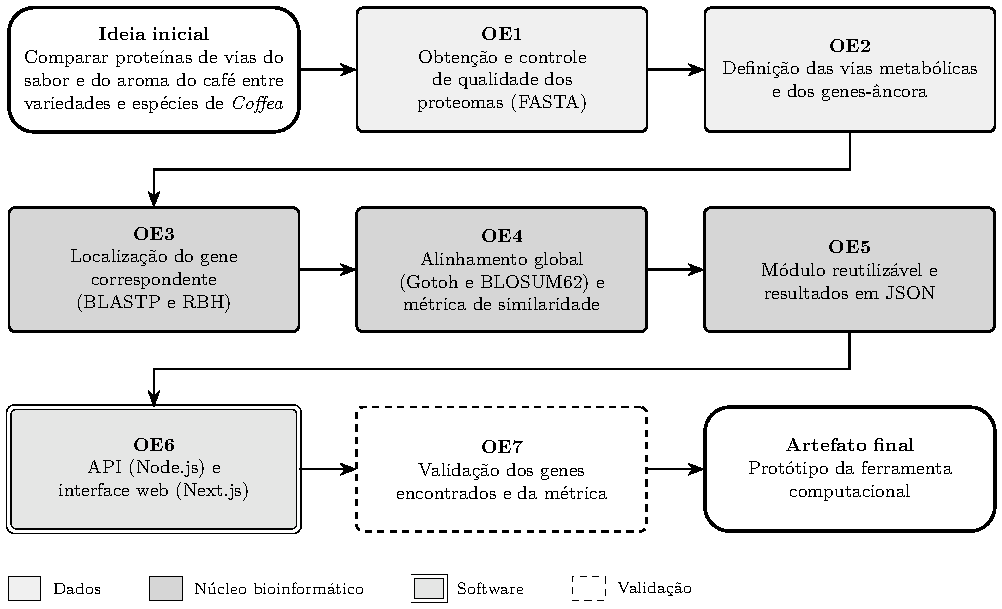
\includegraphics[width=\textwidth]{imagens/diagramaMetodologia}
	\par\vspace{0.2cm}
	\textbf{Fonte:} Elaborada pelo autor
	\label{fig:metodologia}
\end{figure}
\FloatBarrier

\section{Obtenção e Controle de Qualidade dos Dados}

Esta etapa atende ao \ref{oe:dados}. Os proteomas preditos serão obtidos do \textit{Coffee Genome Hub} \cite{Dereeper2015, CoffeeHub}, em arquivos multi-FASTA (Seção~\ref{sec:fasta}). Serão utilizados os proteomas de \textit{C. arabica} Geisha e Red Bourbon, de \textit{C. canephora} DH200-94 e de \textit{C. mauritiana}.

A qualidade de cada proteoma será verificada por quatro indicadores, mensuráveis a partir do arquivo FASTA e do genoma de origem (Seções~\ref{sec:fasta} e \ref{sec:montagem}): o nível de montagem do genoma, a proporção de sequências idênticas, a proporção de resíduos ambíguos (X) e a distribuição do comprimento das proteínas, em especial das muito curtas. Serão exigidos proteomas provenientes de montagens em nível cromossômico e com baixo ruído, pois em montagens fragmentadas genes podem estar ausentes ou incompletos \cite{Alkan2011}.

A versão do genoma e da anotação e a data de obtenção de cada arquivo serão registradas (Seção~\ref{subsec:anotacao}). A leitura dos arquivos e o cálculo dos indicadores serão implementados em Python.

\section{Definição das Vias Metabólicas e das Sequências-Âncora}

Esta etapa atende ao \ref{oe:vias}. A comparação será direcionada a genes de vias metabólicas associadas ao sabor e ao aroma, e não ao proteoma completo. A escolha se justifica por dois motivos: a comparação de genes já caracterizados tem fundamentação biológica explícita, e a comparação entre proteomas completos por melhores correspondências recíprocas tem custo computacional elevado, da ordem de horas por par de genomas em testes preliminares, incompatível com o escopo de um protótipo.

As vias serão a da cafeína (genes \textit{XMT} e \textit{DXMT}, N-metiltransferases), a dos ácidos clorogênicos (gene \textit{HCT}) e a da sacarose (gene \textit{SPS}), descritas na Seção~\ref{sec:cafe} e sintetizadas na Tabela~\ref{tab:vias}. Para cada via, será obtida uma sequência-âncora, isto é, a sequência de proteína de um gene caracterizado na literatura \cite{Uefuji2003, Lallemand2012, Privat2008}, que servirá de consulta para localizar o gene correspondente em cada proteoma. A associação das vias ao sabor e ao aroma é indireta e multifatorial (Seção~\ref{sec:cafe}), de modo que os resultados serão interpretados como comparação de sequências, sem inferência de fenótipo.

\section{Localização do Gene Correspondente}

Esta etapa atende ao \ref{oe:localizacao}. A localização usará o BLAST+ \cite{Camacho2009}, executado localmente. Um banco de dados será construído a partir de cada proteoma, e a sequência-âncora será usada como consulta por BLASTP em cada um deles (Seção~\ref{subsec:blast}). O alinhamento exato por programação dinâmica tem custo proporcional ao produto dos comprimentos das sequências para cada par, o que o torna inviável na busca em bancos de sequências em larga escala; o BLAST, por empregar a heurística de sementes, é a ferramenta padrão da área para essa busca.

A correspondência será confirmada pelo critério de melhores correspondências recíprocas (Seção~\ref{subsec:rbh}): o melhor resultado em cada proteoma será usado como consulta no sentido inverso, e a correspondência será aceita se o melhor resultado dessa busca for o gene de origem da âncora. Para reduzir a escolha de um parálogo, serão aplicados limiares de \textit{E-value} e de cobertura do alinhamento e um filtro adicional de razão de comprimento entre as sequências, pois famílias formadas por duplicações em tandem, como a das N-metiltransferases da cafeína, apresentam várias cópias muito semelhantes (Seções~\ref{subsec:duplicacao} e \ref{subsec:rbh}). Nos genomas de \textit{C. arabica}, que possuem subgenomas, o identificador e o cromossomo de cada gene encontrado serão registrados, para permitir a conferência com a posição esperada.

\section{Alinhamento e Métrica de Similaridade}

Esta etapa atende ao \ref{oe:alinhamento}. O alinhamento entre as proteínas correspondentes será realizado por uma implementação própria, em Python, do algoritmo de \citeauthorandyear{Gotoh1982}, que realiza o alinhamento global com penalidade de lacuna afim (Equação~\ref{eq:gotoh}), com a matriz BLOSUM62 \cite{Henikoff1992}, cujos valores serão lidos por meio do Biopython \cite{Cock2009}. O alinhamento global é adequado a proteínas ortólogas de comprimento semelhante (Seção~\ref{subsec:global}), e as penalidades de abertura e de extensão de lacuna serão parametrizáveis.

Como saída, será calculada a porcentagem de identidade (Equação~\ref{eq:pid}), com $L$ igual ao comprimento do alinhamento, incluindo as lacunas internas (PID1, Tabela~\ref{tab:pid}), acompanhada da cobertura (Equação~\ref{eq:cob}). O denominador será declarado junto a cada valor, pois comprimentos muito diferentes entre as sequências podem reduzir artificialmente a identidade no alinhamento global (Seção~\ref{sec:metricas}).

\section{Organização do Núcleo e Geração dos Resultados}

Esta etapa atende ao \ref{oe:modulo}. Os procedimentos anteriores serão organizados em um módulo Python reutilizável, com funções separadas para a leitura de arquivos FASTA, a localização de correspondências, o alinhamento e a orquestração do fluxo completo. O fluxo será executado para cada via e para cada par de proteomas, o que, com quatro proteomas, resulta em seis pares por via. Os resultados, que incluem os identificadores dos genes, a porcentagem de identidade, a cobertura e os parâmetros utilizados, serão gravados em arquivos JSON. Não será utilizado banco de dados: os arquivos FASTA e os resultados serão mantidos no repositório de controle de versão Git.

\section{API e Interface Web}

Esta etapa atende ao \ref{oe:software}. A camada de software será composta por uma API, em Node.js com TypeScript, que disponibilizará os resultados das comparações, e por uma interface web, em Next.js com React, TypeScript e Tailwind CSS, que permitirá escolher a via e visualizar a similaridade entre os proteomas. As tecnologias empregadas em todo o trabalho estão sintetizadas no Quadro~\ref{qua:ferramentas}. A interface será desenvolvida apenas depois da validação do núcleo, de modo que o desenvolvimento siga a ordem núcleo, API e interface.

\FloatBarrier
\begin{quadro}[!htbp]
	\centering
	\SingleSpacing\footnotesize
	\caption{Tecnologias empregadas em cada componente da ferramenta}
	\begin{tabularx}{\textwidth}{|>{\raggedright\arraybackslash}p{3.4cm}|>{\raggedright\arraybackslash}p{4.4cm}|>{\raggedright\arraybackslash}X|}
		\hline
		\textbf{Componente} & \textbf{Tecnologia} & \textbf{Uso} \\ \hline
		Busca de correspondências & BLAST+ \cite{Camacho2009} & BLASTP local sobre os proteomas \\ \hline
		Núcleo bioinformático & Python e Biopython \cite{Cock2009} & Leitura de FASTA, alinhamento próprio e orquestração; matriz BLOSUM62 \\ \hline
		Servidor & Node.js e TypeScript & API que disponibiliza os resultados \\ \hline
		Interface & Next.js, React, TypeScript e Tailwind CSS & Seleção da via e visualização da similaridade \\ \hline
		Armazenamento & Arquivos FASTA e JSON, com Git & Dados e resultados mantidos no repositório, sem banco de dados \\ \hline
	\end{tabularx}
	\par\vspace{0.2cm}
	\textbf{Fonte:} Elaborado pelo autor
	\label{qua:ferramentas}
\end{quadro}
\FloatBarrier

\section{Validação}

Esta etapa atende ao \ref{oe:validacao}. A validação terá duas frentes. Na primeira, os genes localizados em \textit{C. canephora} serão comparados com os identificadores publicados na literatura para as mesmas proteínas, a fim de verificar se a busca recupera os genes esperados. Na segunda, a implementação do algoritmo de Gotoh será verificada por comparação com uma implementação de referência, em pares de sequências de resultado conhecido. Os valores de identidade obtidos serão interpretados à luz da conservação esperada entre variedades e espécies (Seção~\ref{sec:metricas}) e das diferenças de restrição funcional entre genes (Seção~\ref{sec:evolucao}).